\documentclass[a4paper,10pt]{article}
\usepackage[utf8]{inputenc}
\usepackage{graphicx}


%opening
\title{Physcraper - pipeline for continually updated gene trees}
\author{}

\begin{document}

\maketitle

\begin{abstract}

\end{abstract}

\section{Methods}
The procedure follows 6 steps (Figure 1).\\

\textbf{1) Select an existing phylogeny and alignment}:
This procedure leverages past phylogenetic inference work by relying on existing phylogenies and their associated alignemnts to select appropriate loci to resolve relationships for the taxonomic scope of interest.
Starting from a tree in the Open Tree database, the pipeline automatically searches for the associated alignment using the database link information in the tree metadata. 
%(?? be more specific about Phylesystem not storing alignments and why?!).
The curated trees have information about both rooting and ingroup location. Limiting the sequence search to descendants of the ingroup of the original phylogeny 
and to loci which have been previously vetted by taxon experts reduces the risk of mistakenly inferring homology between paralogous genes or regions and generating spurious results.\\

 \textbf{2)Taxon limited sequence search} 
If the original alignment contains concatenated sequences, the sequences in the alignment are split into individual gene loci.
A sequence search to find homologous sequences within the ingroup's taxon is conducted using each of the alleles in the alignment.
Currently this search uses GenBank.
Alternatively, this approach can utilize whole genome data for adding taxa into gene trees, by treating the observed alleles as tiny provisional reference genomes, 
and assembling homologous loci straight out of whole genome shotgun short read data.\\

\textbf{3) Guided multiple sequence alignment}\\
Starting with an alignment and previously inferred phylogeny simplifies one of the more challenging aspects of automated phylogenetics, multiple sequence alignment.
Multiple sequence alignment is essential to correctly inferring phylogenies, but is in itself based on evolutionary inferences of what nucleotide sites are homologous to one another.
Utilizing an existing estimate of phylogenetic relationships among a subset of the sequences to perform a guided alignment, 
using software such as Pagan (Loytynoja et al., 2012) or PASTA (Mirarab et al., 2015), will improve the speed and accuracy of the overall alignment.

\textbf{4 Placement approach to add novel sequences to existing phylogeny:}\\
Next physcraper applies a placement approach to add the new sequences into the existing tree. 
Placement algorithms allow rapid classification of new samples based on an existing backbone phylogeny.
As this method does not require re-inference of existing branches, it can be very fast.
However, placement approaches do not update existing branches on the tree with respect to information contained in the added taxa,
and do not estimate relationships of the added taxa with respect to one another.
The tree generated by the placement algorithm will be used as a starting tree in a full maximum likelihood or Bayesian tree search.\\

\textbf{5) Perform full maximum likelihood or Bayesian tree search:}\\
Using the placement phylogeny as a starting tree for a new tree search is faster than inferring phylogenies from scratch.
Performing a full tree search will allow relationships that were present in the original tree to change,
as would be expected by the addition of new taxa, and will infer the relationships among the added taxa as well.
The model of evolution for this tree search can be adjusted as parameters change following the addition of sequences.\\

\textbf{6) Repeat:}\\
By repeating the procedure, and continuing to query sequence databases, the pipeline creates a continually updated phylogeny, 
which will provide information about evolutionary relationships as
sequences are added to databases. 

\begin{figure}[!ht]
\begin{center}
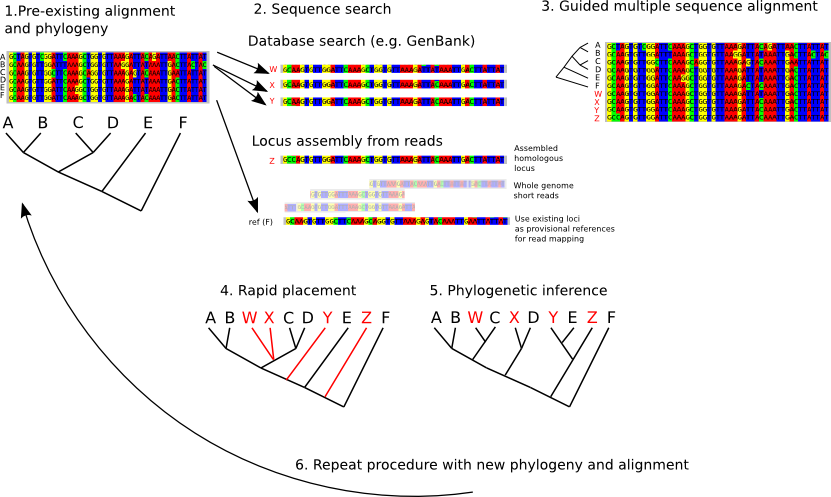
\includegraphics[scale=.65]{physcraper_process.png}
\end{center}
\caption{
 Schematic of phylogenetic updating procedure.}
\label{Figure_label}
\end{figure}


\end{document}
